\chapter{Materials and Methods}

\section{Virus Strains and Passage Histories, By Chapter}

\subsection{Chapter 3: Comparison of Asibi and 17D-204}
The Asibi strain of \gls{yfv} was obtained as lyophilized cell culture supernatant from the \gls{wrceva} (Galveston, TX). The passage history of Asibi strain virus was as follows from the original isolate: six times in rhesus macaque (\emph{Macaca mulatta}) \parencite{Stokes:1928uh}, then 3 times in C6/36 (\emph{Aedes albopictus}) cells. 17D-204 virus was reconstituted from a single, unexpired pharmaceutical dose of lyophilized vaccine (YF-Vax\textsuperscript{\textregistered}, lot number UF795AA, Sanofi Pasteur, USA) using the provided injection diluent. Asibi virus was reconstituted in sterile, deionized water.    
\subsection{Chapter 4: Comparison of 17D Substrain Seeds and Vaccines}
A panel of primary and secondary 17D strain seed lots plus some vaccine production lots was assembled, representing examples of the vaccine lineages 17D-204, 17D-213, and 17DD [Table \ref{origin_seeds}]. Collection strains ampules were obtained as unpassaged, lyophilized stocks from producers, which were reconstituted in molecular grade water for seed ampules or injection diluent for commercial vaccine preparations, without passage. Passage levels were obtained from open literature referencing the strains, with the exception of the 17D-213 substrain vaccine produced in Nigeria, which was of unknown substrain origin and resolved using \gls{blast}. Strains are identified using a nomenclature substrain/origin/lot name/year (year of manufacture is included for strains of same or similar origin).
\subsection{Chapter 5: Comparison of French Neurotropic Vaccine Strains}
\Gls{wt} \gls{fvv} and Asibi strains were obtained from \gls{wrceva} as lyophilized cell culture supernatant. “FNV-IP” was obtained from the Institut Pasteur, (Paris, France). “FNV-Yale” was obtained from the Yale Arbovirus Collection, (New Haven, CT, USA).  “FNV-FC” was obtained from the Centers for Disease Control and Prevention (Fort Collins, CO). “FNV-NT” was obtained from what is now called Public Health England, Porton Down (Salisbury, UK) \parencite{Fitzgeorge:1980vl}. Vaccine strain 17D-204 was obtained from a commercial ampule of YF-Vax\textsuperscript{\textregistered} lot UH356AA (Sanofi-Pasteur, Swiftwater, PA). The passage history of all four \gls{fnv} strains from \gls{fnv} vaccine is unknown but their phenotypic properties have been described \parencite{Wang:1995vu}. All vaccine strains were passaged once only in Vero cells in this study to produce working stocks using Eagle’s minimal essential media, supplemented with 2\% fetal bovine serum (5\% CO$_2$, 37$^{\circ}$C).
\subsection{Chapter 6: Analysis of Subpopulation Selection in a Hamster-Adapted Strain}
The parental Asibi strain was obtained from the \gls{wrceva} (\gls{utmb}, Galveston, TX). Asibi was sequenced without passage by next-generation methods by Beck et. al.; reads were reprocessed for this study \parencite{Beck:2014cm}. Adapted Asibi strain Hamster/P7 was obtained from frozen archived stock as reported by McArthur \parencite{McArthur:2003fv}. Briefly, the virus was passaged from a large plaque variant of the parental strain Asibi (Shope strain as in Chapter 3, \gls{wrceva}, \gls{utmb}) seven times \gls{ip} in Syrian golden hamsters [Figure \ref{Hela_Ham_Derivation}].
\subsection{Chapter 7: Comparison of Wild-Type with Derived Vaccine Strains of Japanese Encephalitis Virus}
The parental \gls{jev} strain SA14 was obtained from a stock passaged once in suckling mouse brain, and then once in Vero cells. Two strains of the SA14-14-2 vaccine were analyzed in the study, the first of which was, from the vaccine ampule, passaged once in C6/36 (\emph{Aedes albopictus}) cells, and is called SA14-14-2/P1. The second analyzed vaccine strain was passaged once in Vero cells from SA14-14-2/P1, and is called SA14-14-2/P2.

\section{RT-PCR}
Viral \gls{rna} was extracted using the QiAmp\textsuperscript{\textregistered} viral \gls{rna} column isolation kit (Qiagen, Gaithersburg, MD). \Gls{rtpcr} amplicons were generated using the listed primers and amplification strategy [Table \ref{tab_NGS_primers}], which were designed in reference to Genbank accession X03700.1, the earliest entry for 17D \parencite{Hahn:1987tw}. Overlapping \gls{rtpcr} amplicons were generated from extracted \gls{vrna} directly, without intervening passage of either virus. Six amplicons were designed to be at least 2 \gls{kb} in size, covering the entire viral genome, with 250b overlap. The amplification program was as follows: reverse transcription for 30 minutes at 50$^{\circ}$C, initial denaturation for 2 minutes at 94$^{\circ}$C, 40 cycles of 10s denaturation at 94$^{\circ}$C, anneal for 30s at a primer-dependent temperature, and extension for 2 minutes at 68$^{\circ}$C. Final extension was at 68$^{\circ}$C for 7 minutes. 
\section{Pipeline}
\subsection{Illumina Sequencing,  \emph{de novo} Assembly, and Preprocessing}
Amplicons were diluted to molar equivalence, and indexed \gls{cdna} libraries generated. Libraries were sequenced on an Illumina Hi-Seq-1000 or 1500 instrument (the instrument upgraded during the course of the dissertation studies), obtaining paired-end, 50b reads. Barcode sequences and three 3’ bases were removed from all reads, retaining those read pairs with average quality scores (Phred scale) above 35. Reads were assembled \emph{de novo} using \index{Software!ABySS}ABySS v.1.3.4, using the paired-end function and k-mer size of 20-40 \parencite{Simpson:2009iv}. Contigs recovered from assembly were screened by \gls{blast} search to detect relative abundance of expected viral templates in the sequencing reaction. Reads were received from the sequencing core lab (\gls{utmb}) as a preliminary assembly against a typical reference, compressed in \gls{bam} format.
\subsection{Reference Sequences and Genome Layouts}
Reference sequences were selected for alignment based on historical reliability, e.g. prototype strains were used for alignment references in all cases.  For chapter 3, the alignment reference was Genbank accession AY640589, a standard reported sequence for Asibi \parencite{McElroy:2005ik}. For chapter 4, the alignment reference was Genbank accession X03700, the original sequence of 17D as reported by Hahn and Rice \parencite{Hahn:1987tw}. For chapter 5, the alignment reference was Genbank accession YFU21056, the wild-type parental \gls{fvv} \parencite{Wang:1995vu}.  For chapter 6, the alignment reference was AY640589. For chapter 7, the alignment reference was Genbank accession JEU14163, a sequence for the wild-type \gls{jev} prototype strain SA14 \parencite{Ni:1994vs}. 

For calling of nucleotide and codon positions of \gls{yfv}, the extent of gene segments was constructed based on inference of typical flavivirus cleavage sites in the \gls{yfv} polyprotein \parencite{Rice:1985tn}. For calling of nucleotide and codon positions in \gls{jev}, the gene segment extents listed by Song, et. al were used \parencite{Song:2012iw}. 

\subsection{Preprocessing and Alignment of Illumina Reads for Downstream Analysis}
The received alignments were disassembled into constituent, paired-end FASTQ files, using the \index{Software!Picard Tools!SamToFastQ}Picard Tools SamToFastq.jar. For reads originating from \gls{rtpcr} amplicons, primer sequences were trimmed from the reads using \index{Software!Trimmomatic.jar}Trimmomatic v.0.30.  Alignment of reads was performed using \index{Software!Picard Tools!SamToFastQ}Bowtie2, in either ``-very-sensitive-local'' or ``-very-sensitive'' modes; the latter use (nonlocal alignment) was only performed for Chapter 3 (Asibi/17D comparison) and Chapter 7 (\gls{jev} comparison) \parencite{Langmead:2012jh}. Alignments were generated in \gls{sam} format first, then compressed to \gls{bam} format and sorted by read nucleotide position using \index{Software!Samtools}samtools/htslib “sort” command \parencite{Li:2009ka}. \Gls{pcr} duplicate removal was performed with \index{Software!Picard Tools!MarkDuplicates}Picard-tools MarkDuplicates.jar, using an optical pixel distance tolerance of 0 (Broad Institute, Cambridge, MA). Read coverage was then measured using the “coverage” command of \index{Software!bamtools}bamtools v.2.4.0. Coverage measurements on processed alignments were used to generate a proportion of mean read coverage in reference to the \gls{bam} alignment file in the experiment (e.g. within a single chapter) with the lowest read coverage after \gls{pcr} duplicate removal; the proportion was used to perform a random downsampling operation on alignments to provide a normalized equalization of coverage for all samples considered in a particular experiment. Downsampling was performed with \index{Software!Picard Tools!DownsampleSam}Picard-Tools DownsampleSam.jar, using the aforementioned normalization ratio to determine random probability of read pair retention (Broad Institute, Cambridge, MA). Final coverage was verified. For Chapter 3 (Asibi/17D comparison), downsampling was performed directly on FASTQ files, before initial alignment, by a custom Python script.

\subsection{Generation and Analysis of Consensus Sequences}
After alignment, \gls{pcr} duplicate removal, and downsampling for coverage  normalization, consensus sequences were generated from coverage-normalized alignments by calls against a pileup file, which was generated using \index{Software!Samtools}samtools v.0.1.9 and \index{Software!Bcftools}bcftools v. 0.1.9, using the biallelic consensus caller of \index{Software!bcftools}bcftools, with base alignment quality filtering disabled for pileup generation. Final sequences were end-padded for end-artifact regions not covered by the sequencing procedure, aligned in reference to the parental sequence in \index{Software!Macvector}MacVector 14.0.1. Substitutions were classified as silent or coding relative to the open reading frame and local codons of the parental strain used in the respective experiment.

\section{Diversity and Divergence of Sequence Alignments}
This section summarizes the use of diversity indices that were used in the studies to estimate both
complexity of the viral populations, and their comparative genetic distance \parencite{Nishijima:2012ew,Li:2010jl}. Nucleotide frequencies were calculated from a matrix of relative nucleotide counts at each nucleotide position, incorporating the four possible nucleotides with a gap symbol that may have been introduces by the aligner. The count matrix was generated using the ``bam2R'' parser in the \index{Software!R}R library \index{Software!R!deepSNV}deepSNV \parencite{Gerstung:2012js}, and then the function ``RF'' of the same library was used to generate an R dataframe of relative nucleotide frequencies per nucleotide site. Diversity index and distance measurements are taken directly from these frequencies
as generated in the \index{Software!R}R environment.

\subsection{Shannon's Entropy}
\index{Formulae!Shannon's Entropy}\Gls{se} $SE$ is calculated for a read alignment at every nucleotide site $X$, summarizing across the entire possible nucleotide mutation set $p$. The probability $P$ is the relative frequency of each possible nucleotide at the position $i$ in the alignment taken as natural logarithm of the same multiplied by the same frequency, which are summed to give a single value for the position. The index can be summarized in multiple ways across
a chosen group or extent of nucleotide positions, usually by descriptive statistics.
	
\begin{align*}
	SE(X)_{ i }=-\sum _{ p=\{ A,T,C,G,-\}  }^{  }{ P[X_{ i,p }]ln(P[{ X }_{ i,p }])}
\end{align*}

Likewise, the \gls{nse} $NSE$ is generated by dividing 1.61, which is the maximum possible $SE$ value for 
the five nucleotide set considered at each position. This reduces the range of the value to zero and 1.00 at minimum and maximum, respectively.	

	\begin{align*}
	NSE(X)_{ i }=-\sum _{ p=\{ A,T,C,G,-\}  }^{  }{ P[X_{ i,p }]ln(P[{ X }_{ i,p }])}/1.61
	\end{align*}

\subsection{Simpson's $1-D$}
\index{Formulae!Simpson's $1-D$}Simpson's $1-D$ is a more stringent value, as the incorporation of zero values in the numerator removes the single-count of the summed nucleotide from the calculation by collapsing it to zero. Similar to $NSE$, the calculation ranges between zero and 1.000 for each nucleotide position considered in a particular alignment, however the natural log transform (as used in $SE$ and $NSE$) is not used as in \gls{se} or \gls{nse}, rendering the calculation less sensitive to changes in frequency at small values. In this case, the value $n$ represents the count of each possible nucleotide at the considered position in the alignment, while $N$ represents the total of those counts for the possible nucleotide set.
	
	\begin{align*}
		S_{1-D}(X)_{ i }=1-\frac{\sum\limits_{p=\{ A,T,C,G,-\}}^{  }n(n-1)}
		{N(N-1)}
	\end{align*}

\subsection{Root-Mean Squared Distance}
\index{Formulae!Root-Mean Squared Distance}\Gls{rmsd} $RMSD$ is calculated using the set $p$ of relative nucleotide frequencies at a chosen nucleotide position in the \gls{bam} alignment. The value accomodates positive and negative movement in frequency for all nucleotides at the position from a baseline alignment $X$ to the frequencies of a resulting alignment $Y$. The value of $RMSD$ increases with genetic distance between the two strain alignments considered. Several landmark values are seen in the calculation, for example 0.632 is the maximum travel of the value, indicating a complete swap of one nucleotide for another.
Half of the maximum, 0.316, is indicative of a selection from an equally diverse state, or equivalent diversification from a completely fixed state.

	\begin{align*}
		RMSD(X, Y)_{ i }=\sqrt{\frac{\sum _{ p=\{ A,T,C,G,-\}  }^{  }{{(P[X_{ i,p }]-P[{ Y }_{ i,p }])}}^2}{5}}
	\end{align*}

\subsection{Error Rate}
\index{Formulae!Error Rate}The sequencing error rate $ER$ estimates the bulk of variant populations in the read alignment at a particular nucleotide position, and includes both true variants as well as false-positive, statistical noise \glspl{snv} introduced by sequencing chemistry or read processing. The value is calculated from the set $p$ of relative nucleotide frequencies at a chosen nucleotide position. By subracting the maximum value in $p$ (the consensus frequency, shown in the inset as $Max(p)$), the resulting value includes the sum of all frequencies not contained in the consensus nucleotide frequency at the considered nucleotide position. Since $ER$ includes both the true variant populations and artifacts, it is useful as a rough estimation of alignment variant distribution before using more rigorous estimates.	

	\begin{align*}
	ER(X)_{ i }=1-Max(p)
	\end{align*}
	
\section{Statistical Methods for Comparison of Sitewise Nucleotide Diversity}
In all studies, diversity and distance indices are compared nonparametrically. For comparisons of entropy, the diversity index is summarized along a selected extent of the genome (whole-genome, open reading frame, individual genes, or selected sets of nucleotide positions) and analyzed using measures of central tendency. To compare the estimate of diversity between two strains, a Kruskal-Wallis/Mann-Whitney test was used with an alpha of 0.05. For comparisons of multiple sequences simultaneously, the Kruskal-Wallis H test was used to perform ommnibus test, with an alpha of 0.05; pairwise comparison of strains was performed with the Wilcoxon Rank-Sum test with Dunn's post-hoc correction of p-values. 

To measure statistically significant changes in nucleotide frequencies between two read alignments, \gls{bam} files were parsed into an R session as nucleotide counts per nucleotide site for all possible values (A, C, G, U, -) and compared using the model of Gerstung and Beerenwinkel (deepSNV) \parencite{Gerstung:2012js}. The model was used with an alpha of 0.05, with a beta-binomial distribution and Bonferroni correction of p-values. The output results from the model indicate nucleotides that have significantly changed in frequency in transition between the two alignments; this may indicate selection, or alternatively may show the presence of \glspl{snv} accurately at low frequency, this depends on the appropriateness of chosen control sample alignment used in the model as a statistical noise floor. For \gls{yfv} 17D and \gls{fnv} strain vaccine samples, the \gls{wt} parental strains Asibi and \gls{fvv} are appropriate choices for control alignments considering the limited number of consensus mutations differentiating them from derived vaccines. 

\section{Resolution and Classification of Single-Nucleotide Variants}
\Glspl{snv} were analyzed from \gls{bam} alignments by two methods. A heuristic analysis was performed (retaining variants above one percent cutoff) by conversion of the \gls{bam} file to pileup format using the \index{Software!Samtools}samtools/htslib “mpileup” command, with base alignment quality filtering disabled. \index{Software!Varscan}VarScan v. 2.3.5 was then used to scan the pileup, retaining variants above one percent. For modeled detection of variants, \index{Software!V-Phaser}V-Phaser v.2.0 was used on the \gls{bam} aligment directly, with default settings and an alpha level of 0.05. Outputs of the variant callers were simplified using GNU \index{Software!GNU Awk}awk 4.1.0, condensing the raw output file(s) into a simplified, delimited table. Variants were classified in reference to the particular consensus sequence generated from the \gls{bam} alignment of each sample, using the Perl script \index{Software!Snpdat.pl}SNPdat.pl \parencite{Doran:2013df}. Classification tables were parsed into \index{Software!R}R sessions and merged with frequency data for graph preparation and depiction using ggplot. 

\subsection{Resolution and Classification of Wild-Type Revertants}
Once generated, the \gls{wt} or parental sequence was scanned in an \index{Software!R}R environment against the table of variants generated by either method. On each cycle of the script, if the variant was a match for the nucleotide identity of the parental sequence and position, it was considered a \gls{wt} revertant. These revertants were classified as coding or silent by virtue of the previous variant detection and classification \emph{in situ}, which was performed by default on each alignment.

\section{Selection Analyses}
\index{Formulae!$dN/dS$}$dN/dS$ ratios were generated by a custom \index{Software!Python}Python script, which incorporates the following series of calculations as described by Morelli \parencite{Morelli:2013jl}. The calculations use the consensus sequence of a chosen \gls{bam} alignment to establish a baseline for mutations detected in the read alignment, and subsequent
generation of the final ratio.

A variable number of nonsynonymous or synonymous mutations may be available at a particular site, which depends on codon type and codon position of the possible mutation(s). These
values $n$ ans $s$ are the number of nonsynonymous and synonymous sites accessible in the reference population, which in this case is the 
consensus sequence of the \gls{bam} alignment used in the analysis. And so, the nonsynonymous sites are calculated over the three codon positions $i$.

	\begin{align*}
	n = \sum _{ {i=1}  }^{3}{f_i}
	\end{align*}

The available synonymous sites $s$ for an individual codon are likewise calculated from the reference by subtraction of $n$.
	
	\begin{align*}
	s=(3-n)
	\end{align*}
	
Nonsynonymous sites $N$ over a particular extent or number of codons in the reference sequence are added.
	
	\begin{align*}
	N = \sum _{ {i=1}  }^{r}{n_i}
	\end{align*}

Synonymous sites $S$ are likewise calculated from the remainder of sites in the extent of the reference considered.	
	
	\begin{align*}
	S=(3r-N)
	\end{align*}

For the sample read alignment $d$ in \gls{bam} format, similar values $N_d$ are calculated for nonsynonymous sites. This analysis requires the scanning
of each read aligned to the region of the reference in the extent of codons from which the analysis is constructed.
	
	\begin{align*}
	N_d = \sum _{ {i=1}  }^{r}{n_{d_i}}
	\end{align*}

Likewise, synonymous sites $S_d$ in the sample to be analyzed are scanned and counted along the extent of the reference used for analysis
, resulting in a summation of silent nucleotide change in the sample region.
	
	\begin{align*}
	S_d = \sum _{ {i=1}  }^{r}{s_i}
	\end{align*}
	
A ratio $P_N$ is expressed between the possible nonsynonymous substitutions in the sample and those detected in the reference.

	\begin{align*}
	P_N = \frac{N_d}{N}
	\end{align*}

Likewise, a ratio $P_N$ is expressed between the possible synonymous substitutions in the reference and those detected in the sample.
	
	\begin{align*}
	P_S = \frac{S_d}{S}
	\end{align*}

The ratio $d_N$ is expressed as a numeric correction of $P_N$.
	
	\begin{align*}
	d_N = -\frac{3}{4}ln(1-{\frac{{4P}_N}{3})}
	\end{align*}

The ratio $D_S$ is expressed as a numeric correction of $P_S$.
	
	\begin{align*}
	d_S = -\frac{3}{4}ln(1-{\frac{{4P}_S}{3})}
	\end{align*}

The final ratio $dN/dS$ is divided out from the previous ratios.
	
	\begin{align*}
	dN/dS = \frac{d_N}{d_S}
	\end{align*}

Calculations were performed with a custom Python script, which processed the reads in two stages. First, all reads in the alignment were scanned to generate a data structure containing the counts of nucleotides contained in the reads at each position in the reference sequence, including the reference identity; this structure was saved in .json format and subsequently used as a count index to generate the actual $dN/dS$ values. Finally, the count index was processed to validate the correct extent of genome segments chosen, and also to summarize the ratio over the extent of the entire genome or discrete genes of the sample. Windowed analysis of $dN/dS$ was performed by calculating the ratio along successive 20-codon windows; this was performed both to resolve selection effects on local domains of the viral genes and to detect smoothing effects caused by broad sampling of the ratio along long gene segments. Peak detection was performed on successive windows by the R package quantmod, with the function ``FindPeaks'' with default settings.

\section{Phylogenetic Methods}
$RMSD$ was used to generate distance phylogenies by generating a matrix of pairwise $RMSD$ between all strain alignments in an experiment. The matrix
of pairwise mean distance was computed over the open reading frames of the strains considered, and used to generate a neighbor-joining distance phylogeny in the R package \index{Software!R!ggthemes}ape, exclusive of any consensus information.

\section{Data Processing Environment and Graphical Methods}
All analysis of genomics datasets was performed on an Intel MacBook Pro (late 2009), using OSX version 10.6 (Snow Leopard) or 10.7.5 (Lion). Package management and version handling for libraries and open-source sequencing applications was performed using \index{Software!Homebrew}Homebrew 0.9.5. Graphs were assembled using the \index{Software!R}R library \index{Software!R!ggplot2}ggplot2, with additional graphical settings provided by the R library \index{Software!R!ggthemes}ggthemes. Tables were constructed in a \LaTeX~environment with the booktabs package.
\clearpage

\begin{sidewaystable}[p]
	\centering
	\caption{Primers for RT-PCR amplifications.}
	\begin{ThreePartTable}
	
		\taburowcolors [2]1{gray!20 .. white}
		% This is the filler table for checking formats.
% Please add the following required packages to your document preamble:
% \usepackage{booktabs}
% Please add the following required packages to your document preamble:
% \usepackage{booktabs}
\footnotesize
	\begin{tabu} to \columnwidth {X[1,l]X[2.5,l]X[.75,l]X[.5,l]X[l]}
			
	\rowfont[1]{\bfseries}
	\toprule
		Primer          & Sequence, 5'--\textgreater3' & Oligo Length(b) & Amplicon Length(b) & Annealing Temperature, $^{\circ}$C \\ \midrule
		17D-1-2005F     & AGTAAATCCTGTGTGCTAATTGAGGTG  & 27              & 2005               & 58.0                      \\
		17D-1-2005R     & GATTGCCGCTGTAAGATCATCAG      & 23              &                    &                           \\
		17D-1749-3725F  & CTGGCGCAATGAGGGTTACAAA       & 22              & 1976               & 58.0                      \\
		17D-1749-3725R  & TTGAAAAGGCAGCAATCAACGC       & 22              &                    &                           \\
		17D-3498-5506F  & GGGTTACAGCTGGAGAAATACATGC    & 25              & 2008               & 59.0\tnote{a}                      \\
		17D-3498-5506R  & ATTTGCCCTAGCTCTGTGCGCT       & 22              &                    &                           \\
		17D-5249-7278F  & GCCCCCACCAGGGTTGTTCTTTCT     & 24              & 2029               & 58.0                      \\
		17D-5249-7278R  & TGCTGCGCTTTGATTCCAGGTA       & 22              &                    &                           \\
		17D-6900-9100F  & TGCTGGAGAAAACCAAAGAGGA       & 22              & 2200               & 58.0                      \\
		17D-6900-9100R  & CTCAAACTCAAGATACCGCGCT       & 22              &                    &                           \\
		17D-8749-10862F & TAGGAAGATCATGAAAGTTGTCAACAGG & 28              & 2113               & 58.0                      \\
		17D-8749-10862R & AGTGGTTTTGTGTTTGTCATCCAA     & 24              &                    &                           \\ \bottomrule
	\end{tabu}

		\begin{tablenotes}
			\item[a]Temperature was used only for chapter with Asibi/17D comparison. All others use 58 degrees C.
		\end{tablenotes}
	\end{ThreePartTable}
	\label{tab_NGS_primers}
\end{sidewaystable}
\clearpage



%\section{Viruses}
%\lipsum[1-2]
%\section{Quantitation of Virus Titers}
%\lipsum[1-2]
%\section{In vitro passage studies}
%\lipsum[1-2]
%\section{Unbiased Handling of Sequencing Data}
%\section{Biased Handling of Sequencing Data}
%\section{Reference Viral Genomes For Data Analysis}
%This will include alignments that refer to the canonical cleavage spots on the genomes,
%and will also include some tables of the lengths of the gene segments and a few domains.
%\subsection{Yellow Fever Virus}
%Include the standard reference genome, and the rationale for choosing it. May also include some
%reference to the strains used in the alignments for each of the studies.
%\subsection{Japanese Encephalitis Virus}
%Include the standard reference genome, and the rationale for choosing it. May also include some
%reference to the strains used in the alignments for each of the studies.
%\lipsum[1-2]
%\clearpage
%
%\subsection{Ribavirin Studies}
%\todo[inline]{Correct the Ribavirin structure, and add the nucleoside for comparison.}
%Ribavirin structure
%\begin{figure}[h]
%	%Source chemfig file for the ribavirin molecule
\chemfig{*5(-O-(-NH2)--)}

%	\caption{Structure of Ribavirin.}
%\end{figure}
%\label{ribavirin}
%%\lipsum[1-2]
%\section{Mouse Studies}
%%\lipsum[1-2]
%
%
%\pagebreak
%\begin{figure}[h]
%	% Tikz flowchart to show the method used in the pipeline of handling the NGS data.

%block styles for the chart.
\tikzstyle{parent} = [rectangle, draw, fill=red!20, 
minimum width=7.2em, align=center, node distance=1cm, minimum height=1.2em, inner sep=0pt]
\tikzstyle{core} = [rectangle, draw, fill=green!20, 
minimum width=7.2em, align=center, node distance=1cm, minimum height=1.2em, inner sep=0pt]
\tikzstyle{clean} = [rectangle, draw, fill=white, 
minimum width=7.2em, align=center, node distance=1cm, minimum height=1.2em,inner sep=0pt]
\tikzstyle{decide} = [rectangle, draw, fill=yellow, 
minimum width=7.2em, align=center, node distance=1cm, minimum height=1.2em,inner sep=0pt]
\tikzstyle{line} = [draw]
\tikzstyle{arrow} = [thick,->,>=stealth,draw]
%\tikzstyle{dashed} = [thick,dashed,draw]

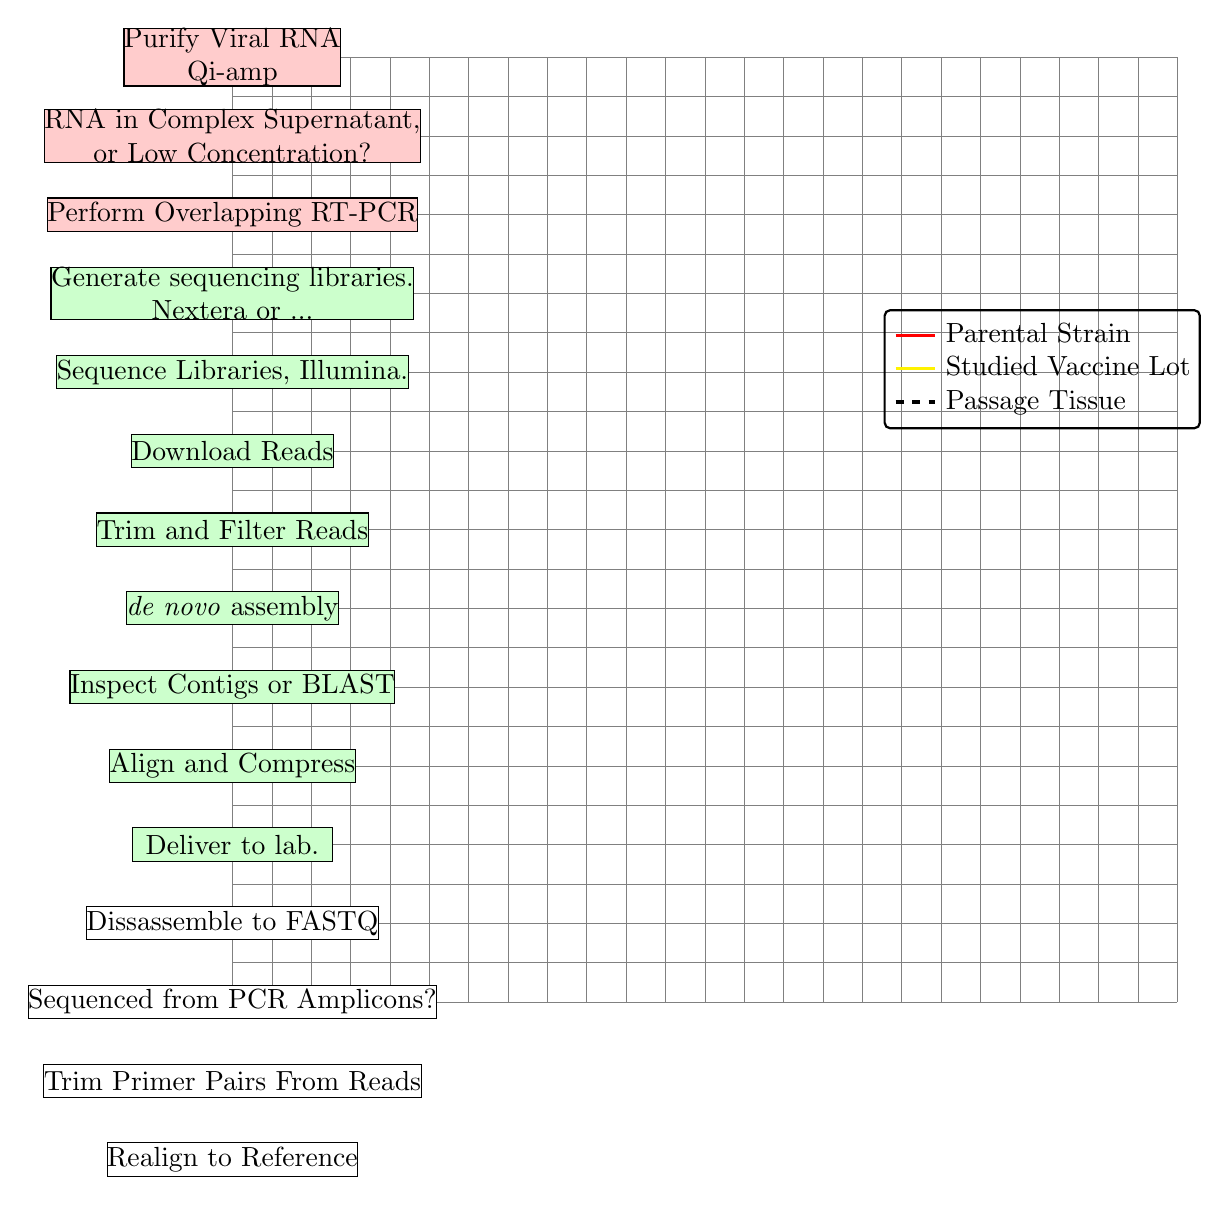
\begin{tikzpicture}[auto]

\draw[help lines,step=.5] (0,0) grid (12,12);

%Nodes for each of the strains mentioned by Yu 2010
% Top
\node[parent](RNA) at (0,12) {Purify Viral RNA \\ Qi-amp};
\node[parent,below of=RNA](isPCR) {RNA in Complex Supernatant,\\ or Low Concentration?};
\node[parent,below of=isPCR](performPCR) {Perform Overlapping RT-PCR};

% Tasks for the Core lab
\node[core, below of=performPCR](library){Generate sequencing libraries.\\Nextera or ...};
\node[core, below of=library](sequence){Sequence Libraries, Illumina.};
\node[core, below of=sequence](download){Download Reads};
\node[core, below of=download](filter){Trim and Filter Reads};
\node[core, below of=filter](assemble){\emph{de novo} assembly};
\node[core, below of=assemble](inspect){Inspect Contigs or BLAST};
\node[core, below of=inspect](align){Align and Compress};
\node[core, below of=align](deliver){Deliver to lab.};

% Tasks after receiving the 
\node[clean, below of=deliver](disassemble){Dissassemble to FASTQ};
\node[clean, below of=disassemble](realign){Sequenced from PCR Amplicons?};
\node[clean, below of=realign](trim){Trim Primer Pairs From Reads};
\node[clean, below of=trim](realign){Realign to Reference};
%
%	
%	%Nodes for each of the three strains considered in the study.
%	\node[studied](TYF2350) at ([xshift=4cm,yshift=-1cm]SA14) {SA14};
%	\node[studied](TYF1454)at ([xshift=4cm,yshift=-0.5cm]SA14-14-2){SA14-14-2};
%	\node[studied, below of=TYF1454](TYF1910){SA14-14-2};	
%	
%	%Arrows connecting the three strains considered in the study.
%	\path[arrow] (SA14-14-2) -| (TYF1454);
%	\path[arrow] (TYF1454) -- (TYF1910);
%	\path[arrow] (SA14) -| (TYF2350);
%	
%	%Arrow connecting Paths
%	\path[arrow] (Mosquito) -- coordinate[midway](M1) (SA14);
%	\path[arrow] (SA14) -- coordinate[midway](M2) (SA14-12-1-7);
%	\path[arrow] (SA14-12-1-7) -- coordinate[midway](M3) (SA14-17-4);
%	\path[arrow] (SA14-17-4) -- coordinate[midway](M4) (SA14-2);
%	\path[arrow] (SA14-2) -- coordinate[midway](M5) (SA14-9);
%	\path[arrow] (SA14-9) -- coordinate[midway](M6) (SA14-9-7);
%	\path[arrow] (SA14-9-7) -- coordinate[midway](M7) (SA14-5-3);
%	\path[arrow] (SA14-5-3) -- coordinate[midway](M8) (SA14-14-2);
%	\path[arrow] (SA14-14-2) -- coordinate[midway](M9) (SA14-14-2-PDK);
%	
%	%Nodes for the passage information
%	\node[information](Mosquito_pass) at ([xshift=-4cm]M1) {11x mb.};
%	\node[information](SA14_pass) at ([xshift=-4cm]M2) {100x PHK, x3 pp. PCE};
%	\node[information](SA14-12-1-7_pass) at ([xshift=-4cm]M3) {2x pp. PCE};
%	\node[information](SA14-17-4_pass) at ([xshift=-4cm]M4) {1x Mouse Spleen(ip.)};
%	\node[information](SA14-2_pass) at ([xshift=-4cm]M5) {3x pp. PCE};
%	\node[information](SA14-9_pass) at ([xshift=-4cm]M6) {1x Mouse Skin};
%	\node[information](SA14-9-7_pass) at ([xshift=-4cm]M7) {6x Hamster Spleen, 2x pp. PHK};
%	\node[information](SA14-5-3_pass) at ([xshift=-4cm]M8) {5x sm. Skin, 2x pp. PHK};
%	\node[information](SA14-14-2_pass) at ([xshift=-4cm]M9) {9x PDK};
%	
%	%Paths connecting passage information nodes with center of arrows.
%	\path[line,dashed] (Mosquito_pass) -- (M1);	
%	\path[line,dashed] (SA14_pass) -- (M2);	
%	\path[line,dashed] (SA14-12-1-7_pass) -- (M3);	
%	\path[line,dashed] (SA14-17-4_pass) -- (M4);
%	\path[line,dashed] (SA14-2_pass) -- (M5);	
%	\path[line,dashed] (SA14-9_pass) -- (M6);	
%	\path[line,dashed] (SA14-9-7_pass) -- (M7);	
%	\path[line,dashed] (SA14-5-3_pass) -- (M8);	
%	\path[line,dashed] (SA14-14-2_pass) -- (M9);	
%	
	
	\node[draw=black,thick,rounded corners=2pt,below left=2mm] at (12.5,9) {%
		\begin{tabular}{@{}r@{ }l@{}}
		%	\raisebox{2pt}{\tikz{\draw[gray, very thick, dashed] (0,0) -- (5mm,0);}}&National Origin\\
		\raisebox{2pt}{\tikz{\draw[red, very thick] (0,0) -- (5mm,0);}}&Parental Strain\\
		\raisebox{2pt}{\tikz{\draw[yellow, very thick] (0,0) -- (5mm,0);}}&Studied Vaccine Lot\\
		\raisebox{2pt}{\tikz{\draw[black,dashed, very thick] (0,0) -- (5mm,0);}}&Passage Tissue\\
		\end{tabular}};	
\end{tikzpicture}
%	\caption{Generalized pipeline for the preparation of NGS datasets, including all steps for 
%		dataset cleanup preceding analysis.}
%\end{figure}
%\label{general_pipeline}
%
%\pagebreak
%\missingfigure[figwidth=\textwidth]{Illustration: NGS data representation.}
%\begin{figure}[h]
%	\input{../ILLUSTRATIONS/Chapter_Methods_ILLUSTRATION/NGS_data_ILLUSTRATION/NGS_data_SOURCE}
%	\caption{NGS data representation.}
%\end{figure}
%\label{NGS_representation}
%
%\pagebreak
%\missingfigure[figwidth=\textwidth]{Illustration: Flowchart for Pipeline 2.}
%\label{Pipeline 2}
%
%
%

%
%
%
%\begin{figure}[h]
%		\caption{RT-PCR schema for overlapping amplicons.}
%		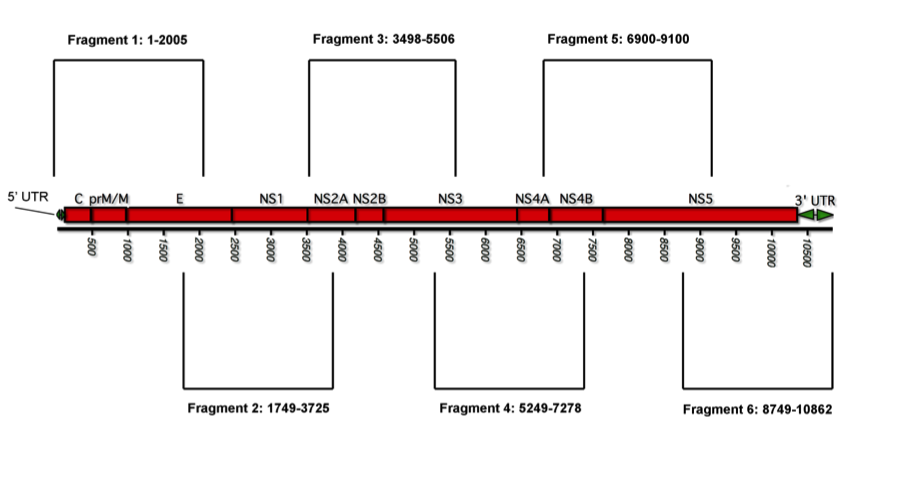
\includegraphics{../FIGURES/Chapter_Methods_FIGURE/PCR_schema/RT_PCR_schema_STANDALONE_1.png}
%		\label{PCR_Schema}
%\end{figure}
%
%\clearpage
%
%\pagebreak
%\missingfigure[figwidth=\textwidth]{Tables: Softwares}
%\begin{table}[h]
%	\centering
%	\caption{Softwares used in the analysis pipelines, with versioning.}
%	\label{my_label}
%	\input{../TABLES/Chapter_Methods_TABLE/NGS_software_TABLE/NGS_software_SOURCE}
%\end{table}
%\label{tab_NGS_software}
%
%\pagebreak
%\missingfigure[figwidth=\textwidth]{Tables: Standard Genomes}
%\begin{table}[h]
%	\centering
%	\caption{Standard Genome annotations for the analyses of YFV and JEV.}
%	\label{my_label}
%	\input{../TABLES/Chapter_Methods_TABLE/NGS_software_TABLE/NGS_software_SOURCE}
%\end{table}
%\label{tab_NGS_software}
%
%\pagebreak
%\missingfigure[figwidth=\textwidth]{Illustration: Diversity measurements}
%\label{Primers}